\documentclass[12pt,aspectratio=43]{beamer}

% 自訂字體的封包
\usepackage{fontspec}

% 導入圖形與表格的封包
\usepackage{graphicx}
\usepackage{booktabs}

% 排列多個子圖形的封包
\usepackage{subfigure} 

 % 提供進階數學環境與公式排版
\usepackage{mathtools, amsmath, amsfonts, amsthm, latexsym} 

%% 設定中文字體
\usepackage{xeCJK}
\setCJKmainfont[AutoFakeBold=3.5 , AutoFakeSlant=0.2]{標楷體}
\setmainfont{Times New Roman}
\XeTeXlinebreaklocale "zh"
\XeTeXlinebreakskip = 0pt plus 1pt

% 自訂字體顏色的封包
\usepackage{color} 

% 圖表自動編號的封包
\usepackage{caption} 

% 允許表格的一格能多列呈現的封包
\usepackage{multirow} 

% 可指定表格排版的封包
\usepackage{array}

% 翻轉表格的封包
\usepackage{lscape} 

% 序列標號
\usepackage{enumerate} 

%% 設定自動編號
\setbeamertemplate{caption}[numbered]

%% 自訂顏色
\definecolor{Myblue}{RGB}{57,108,144}
\definecolor{Default_Blue}{RGB}{52,51,171}

% (動畫)字會若隱若現的顯示
\beamersetuncovermixins{\opaqueness<1->{45}}{\opaqueness<1->{95}} 

% 設定中文的標籤
\renewcommand{\figurename}{圖}
\renewcommand{\tablename}{表}

% 排版形式 
\mode<presentation>{
\usetheme{CambridgeUS}
%	外框形式
\useoutertheme{shadow}
% enumerate 及 item 的形狀
\setbeamertemplate{itemize items}[triangle]
% 調整外框形式的字體大小
\setbeamerfont{headline}{size=\scriptsize}
\setbeamerfont{footline}{size=\scriptsize}
% 取消右下方的跳轉工具列
\setbeamertemplate{navigation symbols}{} 
% 自定義2：清除外框下緣但僅出頁碼
\setbeamertemplate{footline}[page number] 
% 顏色主題
\usecolortheme{dove}
% 設定頁面邊界
\setbeamersize{text margin left=0.2cm, text margin right=0.2cm}
\special{papersize=\the\paperwidth,\the\paperheight}
\providecommand{\tabularnewline}{\\}
}

\title{\fontsize{24pt}{20pt}統計諮詢與專業實務\ 期中}
\author{\fontsize{12pt}{0pt}黃丞暘}
\institute{\fontsize{12pt}{0pt}國立東華大學應用數學統計所}
\date{October 30, 2025}

\begin{document}

% 封面
\begin{frame}
  \titlepage
\end{frame}

% 問題
\begin{frame}[t]{\textbf{問題}} 
\setlength{\parskip}{2pt}
{\Large
  \setlength{\baselineskip}{20pt}
  \parbox{\linewidth}{\raggedright 如何縮短住院天數，並提升病人採用新療法的意願？}}
\begin{itemize}
  \item 目標一：平均住院天數\textbf{降至15天以內}
  \item 目標二：新療法採用率\textbf{相對提升至少25\%}
\end{itemize}
\begin{figure}
  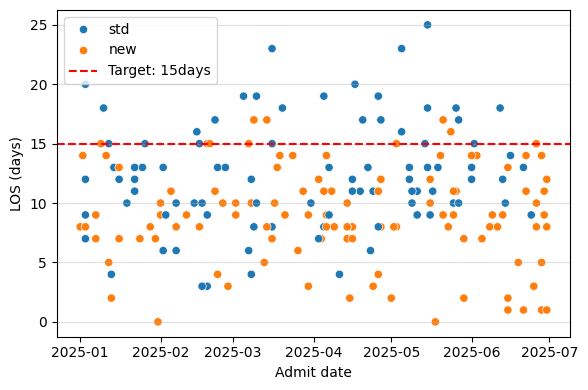
\includegraphics[scale=0.55]{Q.png}
\end{figure}
\end{frame}

% 資料與方法
\begin{frame}{\textbf{資料與方法}}
\linespread{1.5}

\begin{itemize}[]
  \item 研究資料：某醫院所收集的 200 位病人住院紀錄
  \item 研究方法：
  \begin{enumerate}[]
    \item Welch t-test比較新舊療法在住院天數的差異
    \item ANOVA比較合併症程度、年齡區間對住院天數的影響
  \end{enumerate}
  \item 研究流程：
    \begin{figure}
      \hspace{-1cm}
      
\includegraphics[scale=0.8]{流程.png}
    \end{figure}
  
\end{itemize}

\end{frame}

% 結果I
\begin{frame}[t]{\textbf{結果I}}
\setlength{\parskip}{4pt}
{\Large
  \setlength{\baselineskip}{20pt}
  \parbox{\linewidth}{\raggedright 新療法平均住院天數顯著低於舊療法約3.5天}}
    \begin{figure}
      \hspace{25pt}
      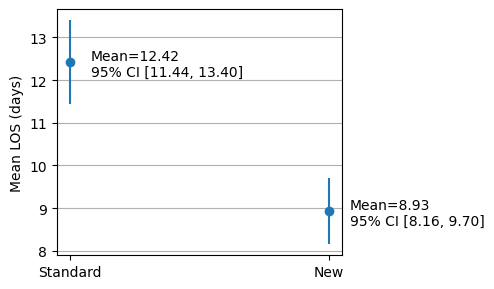
\includegraphics[scale=0.8]{95CI.png}
    \end{figure}
{\small
  \centering 95\% CI = [−4.73, −2.25],　$t = −5.55$,　$p < 0.001$}
\end{frame}

% 結果II
\begin{frame}[t]{\textbf{結果II}}
\setlength{\parskip}{4pt}
{\Large
  \setlength{\baselineskip}{20pt}
  \parbox{\linewidth}{\raggedright 年長且合併症中重度的病人，住院天數明顯更久}}
  \medskip \\
  統計結果顯示年齡與合併症交互作用顯著
    \begin{figure}
      \hspace{-0.5cm}
      
\includegraphics[scale=0.6]{result2.png}
    \end{figure}
\end{frame}

% 建議與改善
\begin{frame}{\textbf{建議與改善}}
\linespread{1.5}

\begin{itemize}
  \item 風險
  \begin{enumerate}
    \item 病人認為醫療費用太高
    \item 新療法設備與技術成本較高
  \end{enumerate}
  \item 建議
  \begin{enumerate}
    \item 用數字說服病人
    \item 進行內部培訓
    \item 配合醫療保險
  \end{enumerate}
  \item 下一步
    \begin{enumerate}
    \item 明年初建立健保給付制度
    \item 積極推廣，6月再評估
  \end{enumerate}
\end{itemize}
\end{frame}

% END
\begin{frame}[plain] % 產生無外框的頁面
	\begin{center}
		{\Huge The End}
		\bigskip\bigskip 
		
		{\LARGE Questions}
	\end{center}
\end{frame}
\end{document}
